%% LaTeX-Beamer template for KIT design
%% by Erik Burger, Christian Hammer
%% edited by Cihat Gündüz, Peter Wolf
%%
%% version 3.0
%%
%% mostly compatible to KIT corporate design v2.0
%% http://intranet.kit.edu/gestaltungsrichtlinien.php
%%
%% Problems, bugs and comments to
%% burger@kit.edu

%% Modified by Sebastian Friebe and Johannes Bechberger

% Selbstdefinierte Kommandos als Arbeitsbeschleunigung:
\newcommand{\f}[1]{\textbf{#1}}					% nutzen in der Form: \f{FETTER TEXT}
\newcommand{\p}{\pause}						% nutzen in der Form: \p (statt \pause}
%\newcommand{\code}[1]{\lstinputlisting[caption=#1]}		% Nutzen in der Form: \code{TITEL}{QUELLE}
\newcommand{\code}[1]{\lstinputlisting[title=#1]}		% Nutzen in der Form: \code{TITEL}{QUELLE}
\newcommand{\cd}[1]{\lstinline[basicstyle=\normalsize\ttfamily]{#1}}		% Nutzen in der Form: \cd{KURZER QUELLTEXT}
\newcommand{\scd}[1]{\lstinline[basicstyle=\scriptsize\ttfamily]{#1}}	% Nutzen in Form: \scd{KLEINER QUELLTEXT} 	% scd steht für Small CoDe
\newcommand{\mcd}[1]{\lstinline[basicstyle=\footnotesize\ttfamily]{#1}}	% für mittlere Größe verwenden!
\newcommand{\bcode}[1]{\lstinputlisting[title=#1,basicstyle=\normalsize\ttfamily]}	% Big Code, Nutzen in der Form: \bcode{TITEL}{QUELLE}
\newcommand{\scode}[1]{\lstinputlisting[title=#1,basicstyle=\tiny\ttfamily]} 	%Small Code, Nutzen in der Form: \scode{TITEL}{QUELLE}

%\newcommand{\trash_to_remove_orange_highlighting}{\end{verbatim}}

\newcommand{\task}[3]{
	\subsection{Aufgabe #1}
	\begin{frame}
		\frametitle{Aufgabe #1}
		#2
		\invisible<1> {
			#3
		}
	\end{frame}

	\begin{frame}
		\frametitle{Aufgabe #1}
		#2
		#3
	\end{frame}
}

\newenvironment{descr}{%
	\newcommand\itemz[2][]{\item[\textbf{##1}] ##2}%
	\begin{description}}{\end{description}%
}

\newenvironment{myitemize}{%
	\newcommand{\conseq}[2][]{\item[\color{kit-green100}\textbf{$\Rightarrow$}] ##2}
	\begin{itemize}}{\end{itemize}%
}

\newcommand{\taskdescr}[3]{
	\task{#1}{
		#2 \\ \vspace{0.2cm}
	}{
		\begin{descr}
		#3
		\end{descr}
	}
}

\newcommand{\taskitemize}[3]{
	\task{#1}{#2}{
	\begin{myitemize}
		#3
	\end{myitemize}
}
}

%% SLIDE FORMAT

\documentclass[18pt]{beamer}

% use 'beamerthemekit' for standard 4:3 ratio
% for widescreen slides (16:9), use 'beamerthemekitwide

\usepackage{templates/beamerthemekit}
% \usepackage{templates/beamerthemekitwide}

% Erlaube Code-Integration mit listings
\definecolor{kit-gray}{RGB}{224,224,224}
\definecolor{kit-green}{RGB}{32,149,128}
\usepackage{listings}
\usepackage{courier}
\usepackage{animate}

\lstset{
         language=C,
%         basicstyle=\scriptsize\ttfamily, % Skriptgröße und Standardschrift
		 basicstyle=\tiny,
         numbers=left,              	% Ort der Zeilennummern
         numberstyle=\tiny,         	% Stil der Zeilennummern
         %stepnumber=2,               	% Abstand zwischen den Zeilennummern
         numbersep=5pt,              	% Abstand der Nummern zum Text
         tabsize=2,                  		% Größe von Tabs
         extendedchars=true,         %
         breaklines=true,            	% Zeilen werden umgebrochen
         %keywordstyle=\color{red},
    	frame=t,         
	%frameround=tftf, 
         keywordstyle=[1]\textbf,    	% Stil der Keywords
         stringstyle=\color{blue}\ttfamily, 	% Farbe der String
         showspaces=false,           	% Leerzeichen anzeigen?
         showtabs=false,             	% Tabs anzeigen?
         showlines=true,              % Leerzeilen am Ende?
         xleftmargin=17pt,
         framexleftmargin=17pt,
         framexrightmargin=6pt,
         framexbottommargin=4pt,
         backgroundcolor=\color{kit-gray},
         commentstyle=\color{kit-green},
         showstringspaces=true    	% Leerzeichen in Strings anzeigen?       
         %numberbychapter=false 
 }

\usepackage{caption}
\DeclareCaptionFont{white}{\color{white}}
\DeclareCaptionFormat{listing}{\colorbox[cmyk]{0.79, 0.18, 0.57,0.03}{\parbox{\textwidth}{\hspace{4pt}#1#2#3}}}
% Taken out since it creats a warning (and I have no idea what it is for)
%\captionsetup[lstlisting]{format=listing,labelfont=white,textfont=white, singlelinecheck=false, margin=0pt, font={bf,footnotesize}}


%% TITLE PICTURE

% if a custom picture is to be used on the title page, copy it into the 'logos'
% directory, in the line below, replace 'mypicture' with the 
% filename (without extension) and uncomment the following line
% (picture proportions: 63 : 20 for standard, 169 : 40 for wide
% *.eps format if you use latex+dvips+ps2pdf, 
% *.jpg/*.png/*.pdf if you use pdflatex)

\titleimage{kit_title}

%% TITLE LOGO

% for a custom logo on the front page, copy your file into the 'logos'
% directory, insert the filename in the line below and uncomment it

\titlelogo{nogo}

% (*.eps format if you use latex+dvips+ps2pdf,
% *.jpg/*.png/*.pdf if you use pdflatex)


% DEUTSCHE SPRACHE EINBINDEN
\usepackage[utf8]{inputenc}

% Deutsche Ausgabe anpassen
\usepackage[T1]{fontenc}

% Für korrekte Unterstreichung etc.
%\usepackage[normalem]{ulem}

% Zeilentrennung
\usepackage[ngerman]{babel}

% disable all navigation symbols
%\beamertemplatenavigationsymbolsempty
% disable only the next-slide, etc, symbols
\setbeamertemplate{navigation symbols}{}

%% TikZ INTEGRATION

% use these packages for PCM symbols and UML classes
% \usepackage{templates/tikzkit}
% \usepackage{templates/tikzuml}

% Only sections in the \tableofcontents
\setcounter{tocdepth}{1}

% Default values
\institute{Lehrstuhl Systemarchitektur}
\title[r3k.vhdl - MIPS R3000 auf dem FPGA]{r3k.vhdl - MIPS R3000 auf einem FPGA}
\author{Aicha Ben Chaouacha, Ahmad Fatoum, Niklas Fuhrberg}


\newcommand\myheading[1]{%
  \par\bigskip
  {\Large\bfseries#1}\par\smallskip}
\setbeamertemplate{caption}{\raggedright\insertcaption\par}
\newcommand{\ebackupbegin}{
   \newcounter{finalframe}
   \setcounter{finalframe}{\value{framenumber}}
}
\newcommand{\ebackupend}{
   \setcounter{framenumber}{\value{finalframe}}
}

\usepackage{color}
\usepackage{listings}
\usepackage{eurosym}
\usepackage{stfloats}
\usepackage{subfig}

\definecolor{javared}{rgb}{0.6,0,0} % for strings
\definecolor{javagreen}{rgb}{0.25,0.5,0.35} % comments
\definecolor{javapurple}{rgb}{0.5,0,0.35} % keywords
\definecolor{javadocblue}{rgb}{0.25,0.35,0.75} % javadoc
\newcommand{\tabitem}{~~\llap{\textbullet}~~}

\lstset{language=C,
	basicstyle=\tiny\ttfamily,
	keywordstyle=\color{javapurple}\bfseries,
	stringstyle=\color{javared},
	commentstyle=\color{javagreen},
	morecomment=[s][\color{javadocblue}]{/**}{*/},
	numbers=none,
	numberstyle=\tiny\color{black},
	stepnumber=1,
	numbersep=0pt,
	tabsize=2,
	showspaces=false,
	showstringspaces=false}

% unten in der preamble.tex sind noch weitere default-werte

\subtitle{Basispraktikum Technische Informatik}
\date{15.08.2017}

% Um das blaue Titel-Bild zu entfernen
%\titleimage{nogo}

\begin{document}

\begin{frame}
	\titlepage
\end{frame}


\section{Unser toller MIPS}

\begin{frame}{Der MIPS R3000}
\begin{itemize}
       \item 1988 auf den Markt gekommen
       \item 32-bit, RISC Architektur
		\item 32 Register
		\item 5-Stufige Pipeline
\end{itemize}


\begin{center}
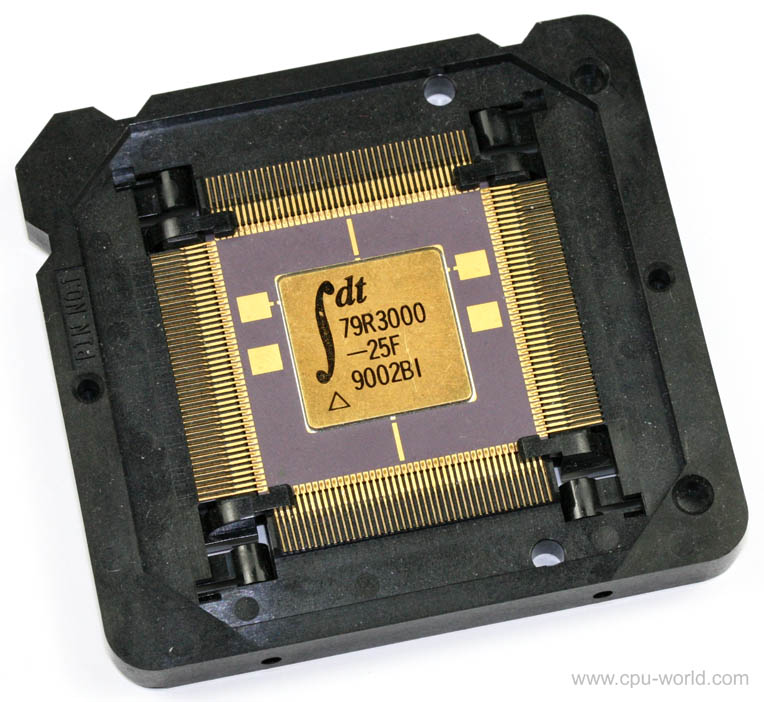
\includegraphics[scale=0.22]{R3000.jpg}
\end{center}

\end{frame}


\begin{frame}[plain]
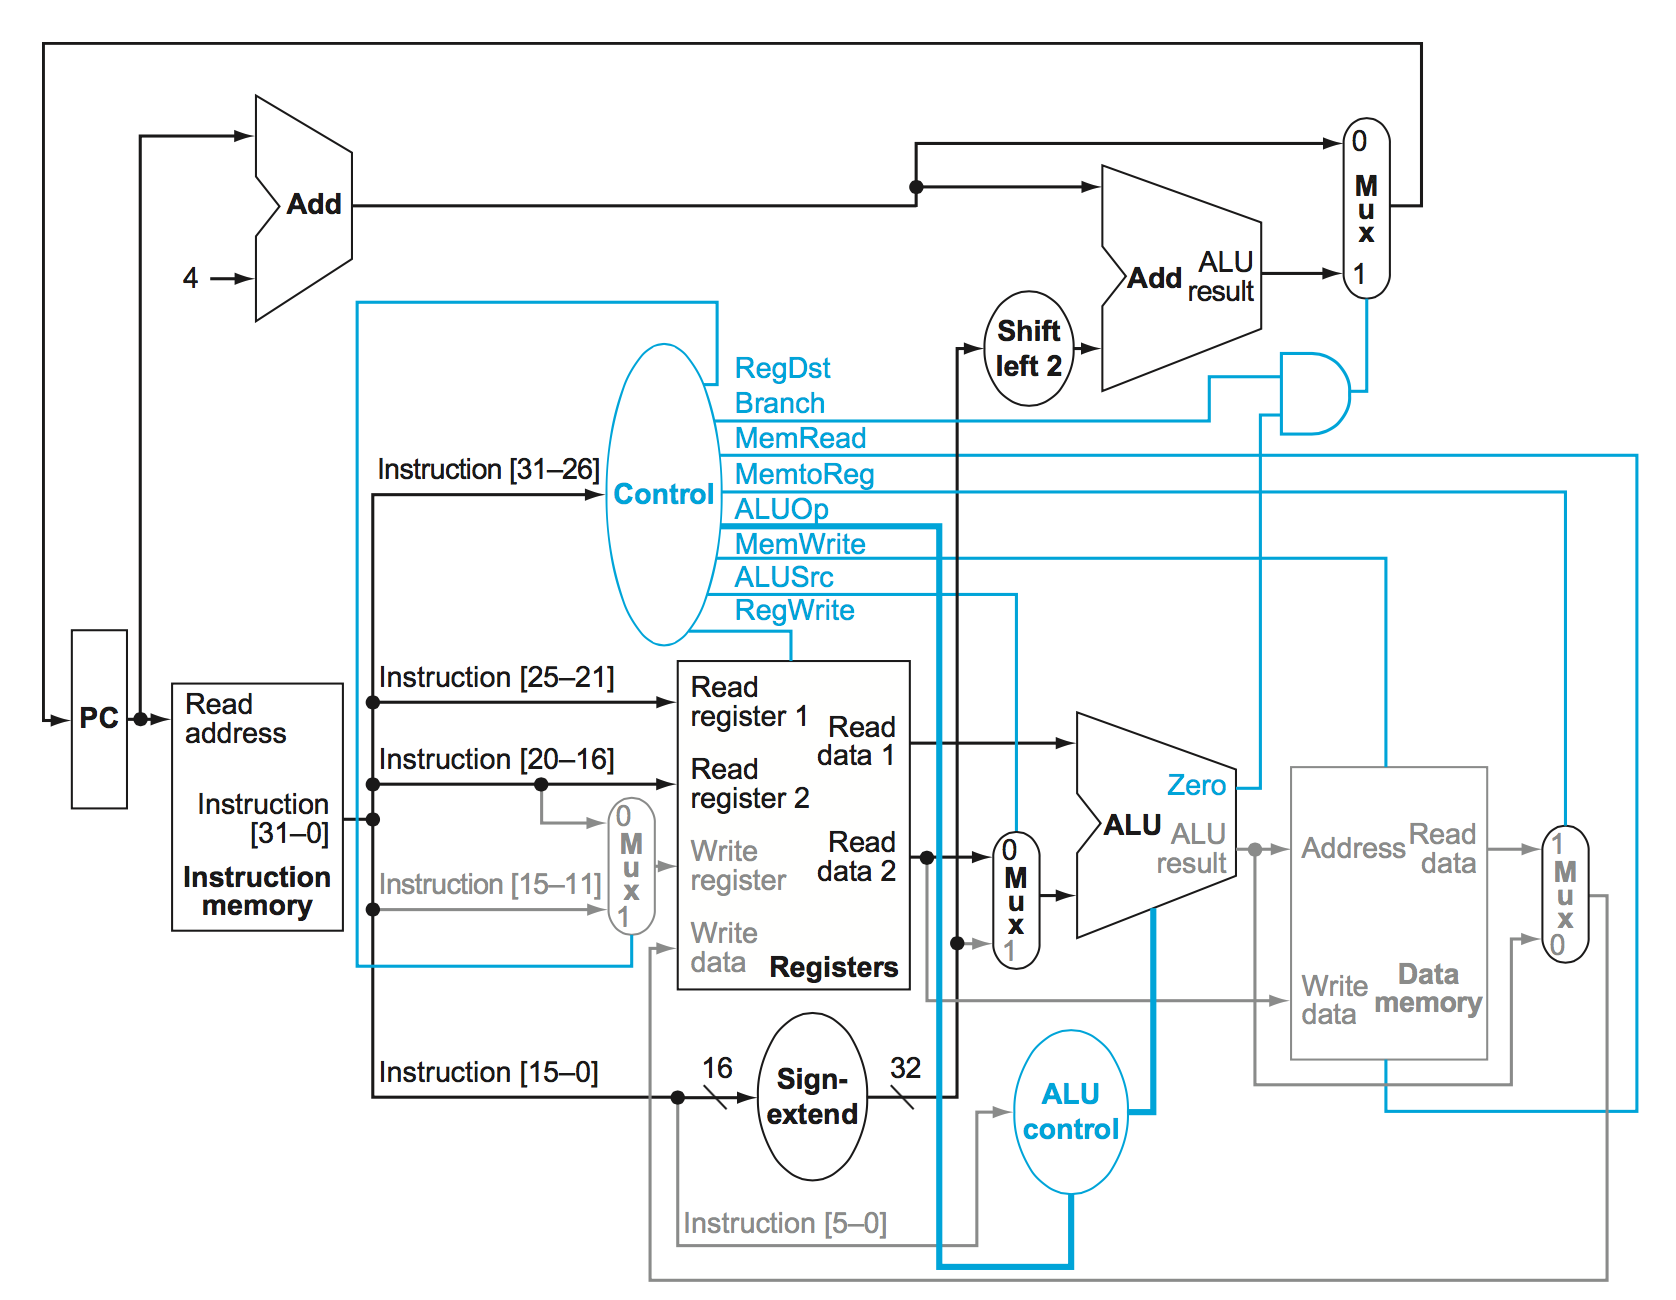
\includegraphics[keepaspectratio=true,width=0.95\paperwidth]{datapath-old.png}
\end{frame}

\begin{frame}[plain]
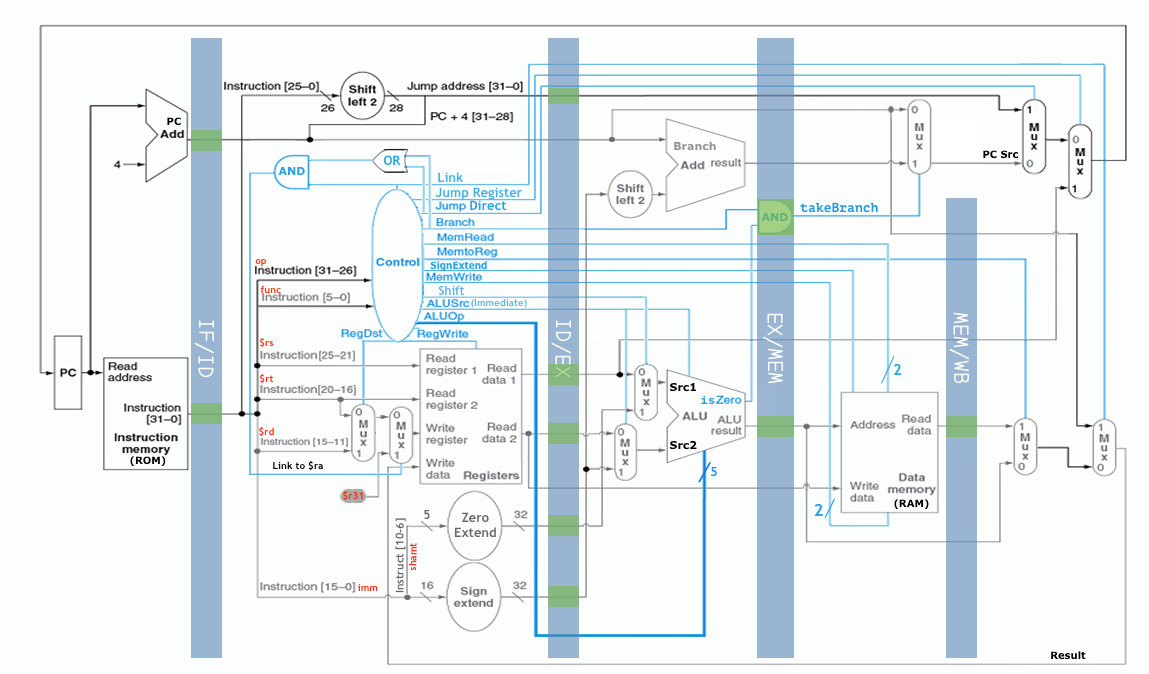
\includegraphics[keepaspectratio=true,width=0.95\paperwidth]{datapath-new.png}
\end{frame}

\begin{frame}{Bus-Teilnehmer}
\begin{itemize}
	\item ROM
	\item RAM
	\item VGA
	\item 8250 UART
	\pause
	\item DIP-Switch \& Buttons
	\item LEDs
\end{itemize}

\begin{center}
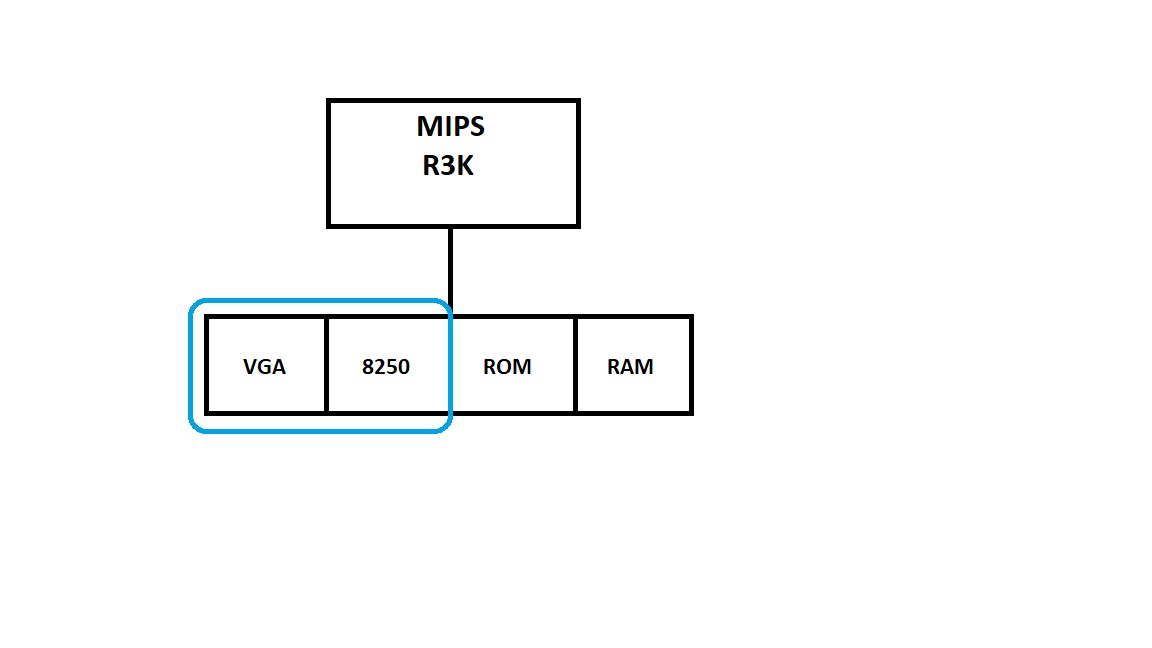
\includegraphics[scale=0.25]{bus.jpeg} %%Grafik s. WA
\end{center}

\end{frame}

\begin{frame}{Memory Map}
\begin{center}
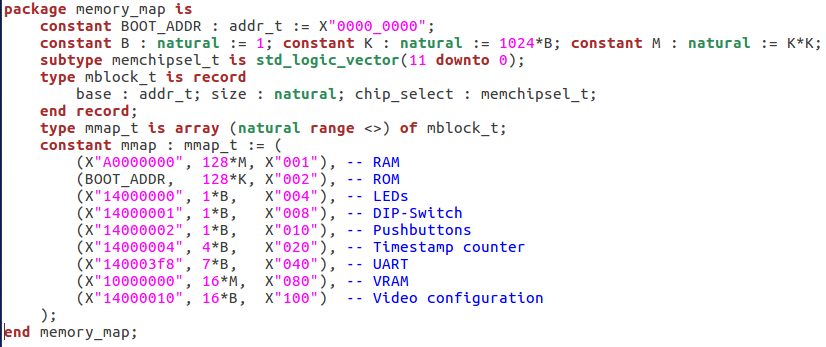
\includegraphics[keepaspectratio=true,width=0.95\paperwidth]{memoryMapPackage.png}
\end{center} 
\end{frame}

\begin{frame}{Memory Interface (Entity)}
\begin{center}
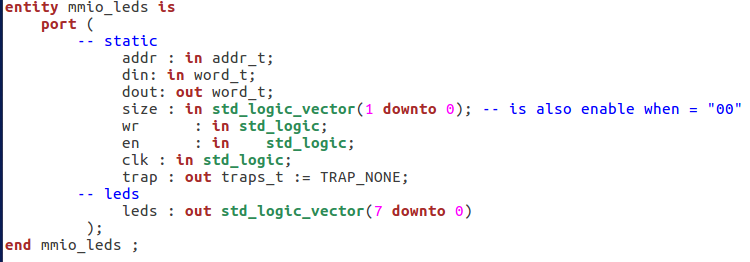
\includegraphics[keepaspectratio=true,width=0.9\paperwidth]{ledsEntity.png}
\end{center} 
\end{frame}

\begin{frame}{LED Architecture}
\begin{center}
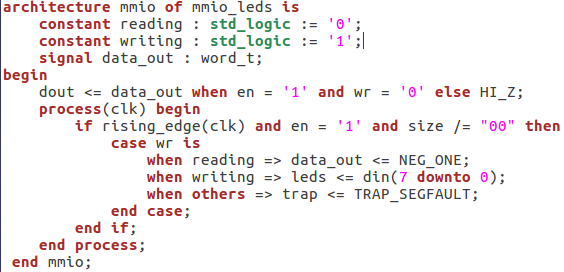
\includegraphics[keepaspectratio=true,width=0.95\paperwidth]{ledsArchitecture.png}
\end{center} 
\end{frame}

\begin{frame}{DIP-Switch Architecture}
\begin{center}
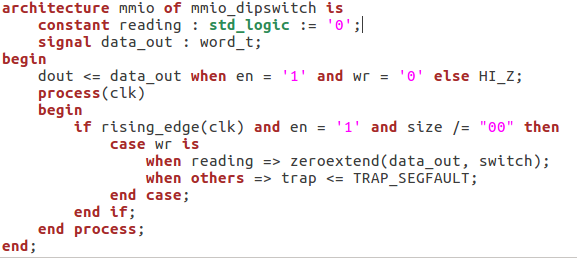
\includegraphics[keepaspectratio=true,width=0.95\paperwidth]{dipswitchArchitecture.png}
\end{center} 
\end{frame}

\begin{frame}{Button to LED}
\begin{center}
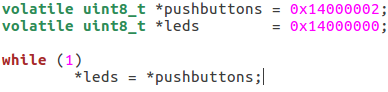
\includegraphics[keepaspectratio=true,width=0.80\paperwidth]{buttonToLed.png}
\end{center} 
\end{frame}

\begin{frame}{Address Decoder}
\begin{center}
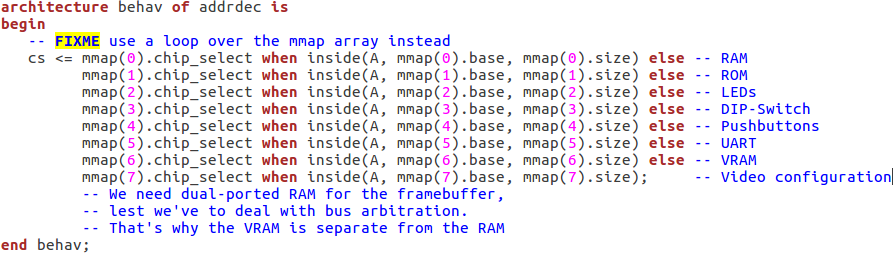
\includegraphics[keepaspectratio=true,width=0.95\paperwidth]{addrdecArichtecture.png}
\end{center} 
\end{frame}

\begin{frame}{VRAM}
\begin{center}
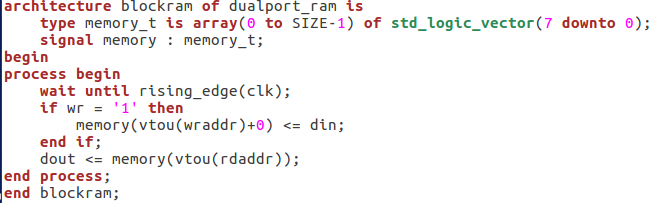
\includegraphics[keepaspectratio=true,width=0.9\paperwidth]{vramArchitecture.png}
\end{center} 
\end{frame}

\section{Unser MIPS System}

\begin{frame}{VGA Frame Puffer (VRAM)}
	\begin{itemize}
		\item C Programm schreibt schreibt in Array
		\item Array wird aus Speicher gelesen
		\item VGA Clock
	\end{itemize}
	\pause
	Realisierung:
	\begin{itemize}
		\item Dual ported memory: Parallele E/A ports mit separaten Clocks
		\item Eine Seite wird über den Memory Bus vom Maschinencode beschrieben
		\item Die andere Seite wird vom VGA Controller gelesen
		\item Separierung in VRAM und VGA Controller
		\item Tupel von VRAM und Controller ist VGA mode. Nur ein Mode implementiert
		\item Überpixel: 32x32 pixel \& 8 bit Farben $\rightarrow$ VRAM-Größe von 300 byte
	\end{itemize}

\end{frame}

\begin{frame}{UART}

\begin{itemize}
	\item Universal Asynchronous Receiver Transmitter
	\item NS8250 Class 
	\item Priorität $\leftarrow$ Erlaubt debugging
	\item keine interrupts
	\pause
	\item Implementiert; aber wegen Zeit/Personalmangel nicht in Betrieb genommen
\end{itemize}
\begin{center}
\end{center}


\end{frame}

\begin{frame}{UART}

\begin{itemize}
	\item Universal Asynchronous Receiver Transmitter
	\item NS8250 Class 
	\item Priorität -> Erlaubt debugging
	\item keine interrupts
	\pause
	\item Implementiert; aber wegen Zeit/Personalmangel nicht in Betrieb genommen
\end{itemize}
\begin{center}
\end{center}


\end{frame}

\section{Verifikation}

\begin{frame}{Testbenches}

\begin{itemize}
\item Emulation:
\begin{itemize}
    \item QEMU mit R3000, UART und VGA
    \item Code lokal Testebar vor Auspielen auf den FPGA
\end{itemize}
    \item Simulation: Testbenches: z.B. ALU und Instruktionsdecoder. Alleinstehend, gut testbar.
\end{itemize}
\begin{center}

\includegraphics[scale=0.85]{qemu.png}
\end{center}

\end{frame}


\begin{frame}{Applikationen}
\begin{itemize}
\item Mandebrot-Fraktal
\item Vllt. DOS Demos portieren
\end{itemize}

\begin{center}

\includegraphics[keepaspectratio=true,width=0.40\paperwidth]{mandelbrot.png}
\end{center}


\end{frame}

\begin{frame}{Fallstudie: DOOM}
       \begin{tabular}{lc}  
         \begin{tabular}{l}
          \parbox{0.5\linewidth}{
          \tabitem ROM: 4 MB benötigt \\
	\tabitem RAM: Block-RAM in Größe von bis zu 19KB verfügbar. DDR-RAM 128MB. 4MB benötigt \\
	\tabitem VRAM: 64,256 byte (320*200, 8 bit Farb Palette) \\
	\tabitem Datentransfer: 5 Minuten bei 115200 baud, wenn keine Bitfehler \\
	\tabitem E/A: Über UART?
}
           \end{tabular}
           & \begin{tabular}{c}
   
\includegraphics[keepaspectratio=true,width=0.38\paperwidth]{doom.png}

         \end{tabular}  \\
\end{tabular}
\end{frame}

\end{document}
